 \documentclass{report}
 \title{IDEA PROPOSAL}	

 \usepackage{graphicx}
 \usepackage{hyperref}

 \begin{document}
 \maketitle
\section{Project Name:}
Forest Conservation Robot
 	
\section{Introduction/Motivation:}
We depend on forests for our survival, from the air we breathe to the wood we use. Wildfire is an important element in biodiversity, but human activity and climate change have caused rapid and dangerous increases in their frequency and intensity worldwide. We are implementing Forest Conservation, robot having functionalities like plant seedling to reforest land, count trees during tree measuring efforts, help prevent and suppress forest fire with forest intelligence system. Robot is autonomously travel In forest through the given specified path and motion feedback sensors. With the help of the fire detection sensor robot detect fire and operator see on live video stream and take action.

\section{Market Research / Literature Survey:}
The existing system are working on satellite feed of forest fire detection and manual seeding to reforest land but the limitation is that the satellite has resolution which is limited to a certain depth of forest so fires below some height cannot be detected also it does not get images when rain or fog is there.
There is no existing robotics system for forest fire detection or forest conservation.

\section{Hardware Requirement:}
\begin{itemize}
	\item Ardiuno UNO R3 
	\item Rasberry Pi
	\item Wifi module
	\item GSM module
	\item IMU Sensors
	\item Ultrasonic Sensor
	\item Temperature Sensor
	\item Humidity Sensor
	\item Fire detection Sensor
\end{itemize}

\section{Software Requirement:}
\begin{itemize}
	\item Ardiuno IDE
	\item Miniconda
	\item OpenCV
\end{itemize}

\section{Implementation:}

\begin{figure}
	\centering
	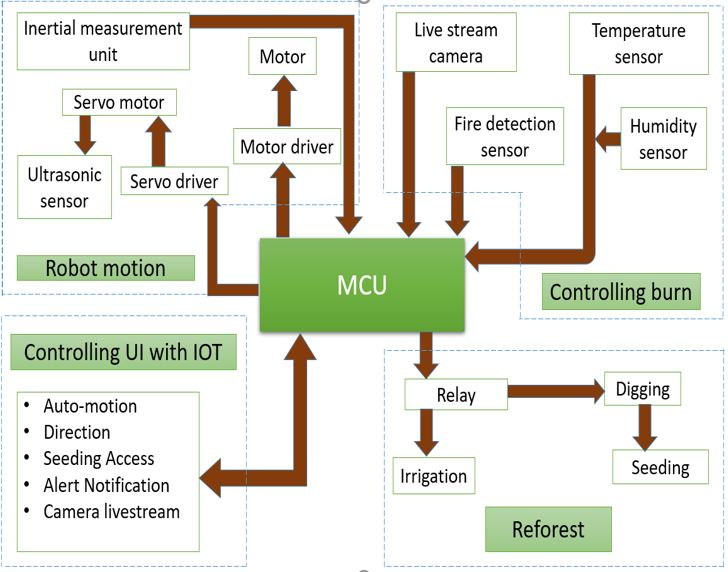
\includegraphics{implementation1.jpg}
	\caption{Block Diagram}
	\label{image_1} % Label is used for referencing
\end{figure}

As shown in block diagram, the complete system can be divided into main four functional units such as Controlling UI with IOT, Robot motion, Controlling burn and Reforest.
The control unit (MCU) includes a Wi-Fi for IOT. IOT is used to give input parameters to MCU to operate Robot. The input parameters are Direction, speed, digging, seeding, water. The MCU plays vital role in the proposed system. The MCU is programmed to control all sensors and relays which operate DC motors, servo motor through servo driver.
The Robot motion involves motors, shaft, wheels, motor driver, Inertial measurement unit, Ultrasonic sensor, Servo motor, Servo driver.
The controlling burn involves fire detection sensor, humidity sensor, temperature sensor, and also accuracy of the robot having addition feature live camera stream. 
The Reforest is semi-autonomous process which involves relay, digging, seeding, water for seed.

\begin{figure}
	\centering
	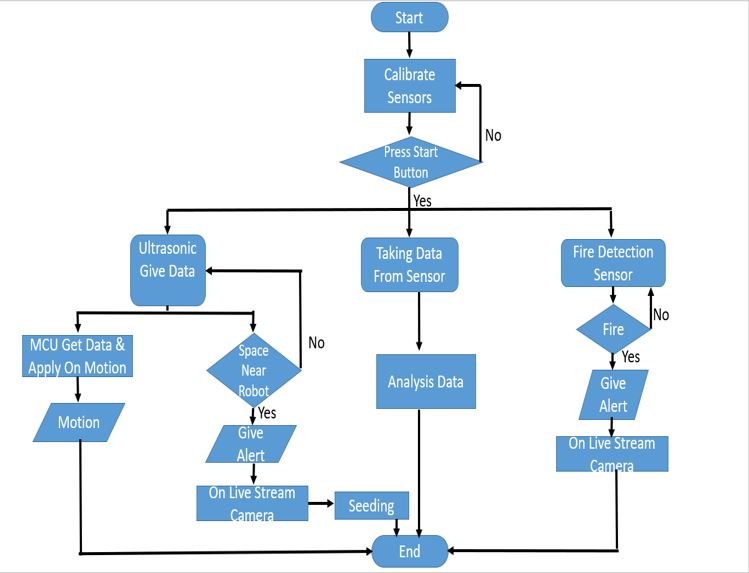
\includegraphics{implementation2.jpg}
	\caption{Flow Diagram}
	\label{image_2} % Label is used for referencing
\end{figure}

Once the MCU is commanded to start, the DC motor coupled is given supply and controlled with the help of motor driver to give smooth motion in forest.
Once the ultrasonic sensor senses the presence of space then MCU send alert message to operator. Operator is verify using live camera stream, after the operator permission seeding is start. That process is autonomous.
The other sensors like humidity, temperature, fire detect are to detect and analyze fire.
With the help of sensor fire is detect then MCU send alert message to operator. Operator verify through live camera stream.
Through the help of feedback system like, Inertial measurement unit, Ultrasonic sensor. Robot is Autonomously travel in forest.
In some of the critical  situation robot is manually operated by operator.

\section{Feasibility:}
The existing system are working on satellite feed of forest fire detection and manual seeding to reforest land but the limitation is that the satellite has resolution which is limited to a certain depth of forest so fires below some height cannot be detected also it does not get images when rain or fog is there.
To overcome the limitations in existing system we have come up with an idea of an Automatic robot which can go through any path and area of forest and efficiently detect forest fires as well as land for reforestation to increase green cover.

\section{References:}
\begin{enumerate}
	\item http://fsi.nic.in/limitations
	\item https://www.replacedbyrobot.info/70288/forest-and-conservation-workers
	\item https://www.iii.org/fact-statistic/facts-statistics-wildfires
\end{enumerate}
 \end{document}